\documentclass{article}

\usepackage{amsfonts}
\usepackage{amsthm}
\usepackage{amsmath}
\usepackage{amssymb}
\usepackage{upgreek}
\usepackage[cm]{fullpage}
%%\usepackage{algorithmic}
%%\usepackage{algorithm} % must read after hyperref
\usepackage[colorlinks={true}, citecolor=blue, linkcolor=blue]{hyperref}       % hyperlinks
\usepackage{algpseudocode}
\usepackage{bbm}
\usepackage{bm}
\usepackage{graphicx}
\graphicspath{{./img/}}
\newtheorem{proposition}{Proposition}

%% \usepackage{array}
%% \usepackage{comment,array,wasysym}
%% \usepackage{graphicx,color,colortbl}

%% % \usepackage{mathptmx} % Use Times as default text font, and provide maths support.  I hate what it does to mathcal so I comment it out
%% % \usepackage{mathtools}
%% % \usepackage{multimedia}
%% % \usepackage{subfigure}
%% %\usepackage{ulem} % for strikethrough \sout
%% \usepackage[normalem]{ulem} % for strikethrough \sout, but avoid the annoying underline in \emph



%% % 
%% % \usepackage[utf8x]{inputenc}
%% % \usepackage{default}

%% % AISTATS sty file doesn't play nicely with caption and subcaption pkgs
%% % \usepackage{caption} 
%% %\usepackage{subcaption}

%% \usepackage{caption}
%% \DeclareCaptionType{copyrightbox}  % Without this, the AISTATs sty creates some clash
%% \usepackage{subcaption}


%% \usepackage{ifthen}
%% \usepackage{enumerate}


%% % 
%% % 
%% %         
%% % \usepackage{yhmath}  % I want really wide tilde. Oren Freifeld, 05/19/2013       




%% %% ICML PACKAGES %%
%% %% \usepackage{ellipsis}

%% %% \usepackage{multirow}

%% %% % Recommended, but optional, packages for figures and better typesetting:
%% %% \usepackage{microtype}
%% %% \usepackage{graphicx}
%% %% % \usepackage{subfigure}
%% %% \usepackage{booktabs} % for professional tables

%% %% % hyperref makes hyperlinks in the resulting PDF.
%% %% % If your build breaks (sometimes temporarily if a hyperlink spans a page)
%% %% % please comment out the following usepackage line and replace
%% %% % \usepackage{icml2018} with \usepackage[nohyperref]{icml2018} above.
%% %% \usepackage{hyperref}

%% %% % Attempt to make hyperref and algorithmic work together better:
%% %% \newcommand{\theHalgorithm}{\arabic{algorithm}}


%% %
%% % Commenting macros
%% %
%% \newcommand{\BLUE}[1]{{{\color{blue}{#1}}}}      
\newcommand{\RED}[1]{{{\color{red}{#1}}}}     
%% \newcommand{\MAGENTA}[1]{{{\color{magenta}{#1}}}}     
%% \definecolor{darkgreen}{rgb}{0,.5,0 }
%% \newcommand{\DARKGREEN}[1]{{{\color{darkgreen}{#1}}}}      
%% \newcommand{\TBD}{\RED{[--TBD--]}}
%% \newcommand{\TODO}[1]{\RED{[--TODO: #1--]}}
%% \newcommand{\BRAINDUMP}[1]{\DARKGREEN{[BRAIN DUMP: #1]}}
%  
%  \newcommand{\OREN}[1]{\RED{[Oren says: #1]}}
% % PICK YOUR COLOR...
\newcommand{\jwf}[1]{\BLUE{<\textbf{JWF}: #1 >}}
% \newcommand{\SUE}[1]{\MAGENTA{[Sue says: #1]}}

% MRF
\newcommand{\pot}{\psi}
\newcommand{\epmarg}{q}
\newcommand{\logpart}{\Phi}

% min / max
\DeclareMathOperator*{\argmax}{arg\,max\;}
\DeclareMathOperator*{\argmin}{arg\,min\;}

% Info Theory Stuff
\newcommand{\KL}[2]{\mathrm{KL}(#1\,\|\,#2)}

%
% List macros
%
\newcommand{\bi}{\begin{itemize}}
\newcommand{\ei}{\end{itemize}}
\newcommand{\deriv}{\mathrm{d}}

\newcommand{\etal}{\textit{et al}}
\newcommand{\FIG}{Fig.~}
%\newcommand{\FIGS}{Figs.~}

 \newcommand{\SEC}{Sec.~}

\newcommand{\eg}{\textit{e.g.}~}
\newcommand{\ie}{\textit{i.e.}~}
\newcommand{\cf}{\textit{c.f.}~}


\newcommand{\EQN}{Eqn.~}
% \newcommand{\EQN}{Equation }
\newcommand{\EQNS}{Eqns.~}
% \newcommand{\EQNS}{Equations }

% Expectation and Probability
\newcommand{\EE}{\ensuremath{\mathbb{E}}}
\newcommand{\PP}{\ensuremath{\mathbb{P}}}


% distributions
\newcommand{\Dir}{\ensuremath{\text{Dirichlet}}}
 
% integers
\newcommand{\ZZ}{\ensuremath{\mathbb{Z}}}
\newcommand{\RR}{\ensuremath{\mathbb{R}}}
\newcommand{\Rtwo}{\ensuremath{\RR^2}}
\newcommand{\Rthree}{\ensuremath{\RR^3}}
\newcommand{\Rn}{\ensuremath{\RR^n}}
% 
%positive integers
\newcommand{\Zplus}{\ensuremath{\ZZ^+}}
%positive reals
\newcommand{\Rplus}{\ensuremath{\RR^+}}


% n by n matrices
\newcommand{\nBynMats}{\ensuremath{\RR^{n \times n}}}
% m by n matrices
\newcommand{\mBynMats}{\ensuremath{\RR^{m \times n}}}
% n by p matrices
\newcommand{\nBypMats}{\ensuremath{\RR^{n \times p}}}
% 2 by 2
\newcommand{\TwoByTwoMats}{\ensuremath{\RR^{2 \times 2}}}
% 3 by 3
\newcommand{\ThreeByThreeMats}{\ensuremath{\RR^{3 \times 3}}}
% 2 by 3
\newcommand{\TwoByThreeMats}{\ensuremath{\RR^{2 \times 3}}}




% \newcommand{\EqualsDef}{\,{\overset{\text{def}}{=}}\,}
\newcommand{\EqualsDef}{\triangleq}


% set notation
% \newcommand{\set}[1]{\ensuremath{{\left\{#1\right\}}}}
\newcommand{\set}[1]{\ensuremath{{\{#1\}}}}


\newcommand{\InnerProduct}[2]{\left\langle #1,#2 \right\rangle}

\newcommand{\norm}[1]{{{\left\|#1\right\|}}}
\newcommand{\sign}[1]{{\mathrm{sign}\left(#1\right)}}


\newcommand{\ellTwoNorm}[1]{\norm{#1}_{\ellTwo}}


\newcommand{\Acal}{\mathcal{A}}
\newcommand{\Bcal}{\mathcal{B}}
\newcommand{\Ccal}{\mathcal{C}}
\newcommand{\Dcal}{\mathcal{D}}
\newcommand{\Ecal}{\mathcal{E}}
\newcommand{\Fcal}{\mathcal{F}}
\newcommand{\Gcal}{\mathcal{G}}
\newcommand{\Mcal}{\mathcal{M}}
\newcommand{\Ncal}{\mathcal{N}}
\newcommand{\Ocal}{\mathcal{O}}
\newcommand{\Pcal}{\mathcal{P}}
\newcommand{\Qcal}{\mathcal{Q}}
\newcommand{\Tcal}{\mathcal{T}}
\newcommand{\Ucal}{\mathcal{U}}
\newcommand{\Vcal}{\mathcal{V}}
\newcommand{\Wcal}{\mathcal{W}}
\newcommand{\Xcal}{\mathcal{X}}
\newcommand{\Ycal}{\mathcal{Y}}

\newcommand{\MATRIX}[2][cccccccccccccccccccc]{\left[
 \begin{array}{#1}
 #2
 \end{array}
\right]}


\newcommand{\TRACE}{\mathrm{trace}}

\newcommand{\var}[1]{\text{var} \big( #1 \big) }
\newcommand{\cov}[2]{\text{cov} \big( #1,#2 \big)}
\newcommand{\myt}[1]{\widetilde {#1} }

% bold font math 
\bmdefine\balpha{\alpha}
\bmdefine\bbeta{\beta}

\bmdefine\bphi{\phi}


\bmdefine\bb{b}

\bmdefine\bx{x}
\bmdefine\by{y}
\bmdefine\bdotx{\dot{x}}
\bmdefine\bxzero{x_{0}}
\bmdefine\bxone{x_{1}}

\bmdefine\bu{u}

\bmdefine\bv{v}
\bmdefine\br{r}


\bmdefine\bA{A}
\bmdefine\bB{B}

\bmdefine\bS{S}

\bmdefine\bU{U}

\bmdefine\bV{V}
\bmdefine\bX{X}
\bmdefine\bY{Y}


%\bmdefine\balpha{\alpha}

 \newcommand{\Nc}{{N_{c}}}
% \newcommand{\Nc}{N}
\newcommand{\Ne}{{N_{e}}}

% homo coo
\newcommand{\bxh}{\widetilde{\bx}}




\newcommand{\GLn}{\ensuremath{\mathrm{GL(n)}}}
\newcommand{\gln}{\ensuremath{\mathfrak{gl(n)}}}

\newcommand{\GLone}{\ensuremath{\mathrm{GL(1)}}}
\newcommand{\GLtwo}{\ensuremath{\mathrm{GL(2)}}}
\newcommand{\glTwo}{\ensuremath{\mathfrak{gl}(2)}}


% CPA Stuff

\newcommand{\Ac}[1]{A_{c(#1)}}
\newcommand{\Bc}[1]{B_{c(#1)}}

\newcommand{\Vaff}{\Vcal_{\mathrm{aff}}}

\newcommand{\Vpa}{\Vcal_{\mathrm{PA}}}
\newcommand{\Vcpa}{\Vcal_{\mathrm{CPA}}}


\newcommand{\Faff}{\Fcal_{\mathrm{aff}}}

\newcommand{\Fpa}{\Fcal_{\mathrm{PA}}}
\newcommand{\Fcpa}{\Fcal_{\mathrm{CPA}}}

\newcommand{\NSTEPS}{N_{\mathrm{STEPS}}}
\newcommand{\nsteps}{n_{\mathrm{steps}}}


\newcommand{\SigmaPA}{\Sigma_{\mathrm{PA}}}

\newcommand{\SigmaCPA}{\Sigma_{\mathrm{CPA}}}



\newcommand{\Vat}[1]{\bv{(#1)}}
\newcommand{\VatX}{\Vat{\bx}}
\newcommand{\Tat}[2]{T{(#1,#2)}}
\newcommand{\Tinvat}[2]{T^{-1}{(#1,#2)}}
\newcommand{\VatT}[1][t]{\Vat{\Tat{\bx}{#1}}}
% \newcommand{\VatT}[1][t]{\Vat{\Tat{\bx,#1}}}
\newcommand{\VatTinv}[1][t]{\Vat{\Tinvat{\bx}{#1}}}


\newcommand{\IntVatTofX}[1][t]{\int_{0}^{#1}\VatT[\tau]\, d\tau}

\newcommand{\AtimesX}{A{\bxh}}
 

\newcommand{\CpaVatX}{\Ac{\bx}\bxh}
% \newcommand{\CpaVatT}[1][t]{\Ac{\Tat{\bx}{#1}}\widetilde{T}(\bx,#1)}
\newcommand{\CpaVatT}[1][t]{\Ac{\Tat{\bx}{#1}}\widetilde{\Tat{\bx}{#1}}}

\newcommand{\IntCpaVatT}[1][t]{\int_{0}^{#1} \CpaVatT[\tau] \, d\tau}


 

\newcommand{\IntCpaVatTinv}[1][t]{\int_{0}^{#1}  \Ac{\Tinvat{\by}{#1}}\widetilde{\Tinvat{\by}{#1}} \, d\tau}


\newcommand{\CpaVatXasLinComb}{\sum_{j=1}^{d}\alpha_k\Bc{\bx}^{j}\bxh}
\newcommand{\CpaVatTasLinComb}[1][t]{\sum_{j}^{d}\alpha_j\Bc{\Tat{\bx}{#1}}^{j}\widetilde{\Tat{\bx}{#1}}}


\newcommand{\IntCpaVatTLinComb}[1][t]{\int_{0}^{#1}  \CpaVatTasLinComb[\tau] \, d\tau}


% USAGE:
% $\Vat{\bx}$
% $\VatX$
% $\Tat{\bx}{t}$
% $\VatT$
% $\VatT[\tau]$
% $\VatTinv[\tau]$
% $\IntVatTofX$
% $\AtimesX$
% $\Ac{\bx}$
% $\CpaVatX$
% $\IntCpaVatT$
% $\CpaVatXasLinComb$
% $\IntCpaVatTLinComb$



%\newcommand{\VEE}[1]{{#1}^{\vee}}
\newcommand{\VEE}[1]{\mathrm{vec}({#1})}

\newcommand{\HAT}[1]{{#1}^{\wedge}}

 \newcommand{\LCONSTRAINTS}{L_{\mathrm{constraints}}}

% Graph stuff
\newcommand{\parent}{\text{Pa}}
\newcommand{\interventions}{\mathcal{I}}
\newcommand{\alldata}{\mathcal{X}}

% Planning stuff
\newcommand{\actionset}{\mathcal{A}}


% if you need to pass options to natbib, use, e.g.:
% \PassOptionsToPackage{numbers, compress}{natbib}
% before loading nips_2018

% ready for submission
\usepackage[preprint]{nips_2018}

% to compile a preprint version, e.g., for submission to arXiv, add
% add the [preprint] option:
% \usepackage[preprint]{nips_2018}

% to compile a camera-ready version, add the [final] option, e.g.:
% \usepackage[final]{nips_2018}

% to avoid loading the natbib package, add option nonatbib:
% \usepackage[nonatbib]{nips_2018}

%% \usepackage[utf8]{inputenc} % allow utf-8 input
%% \usepackage[T1]{fontenc}    % use 8-bit T1 fonts
%% \usepackage{hyperref}       % hyperlinks
%% \usepackage{url}            % simple URL typesetting
%% \usepackage{booktabs}       % professional-quality tables
%% \usepackage{amsfonts}       % blackboard math symbols
%% \usepackage{nicefrac}       % compact symbols for 1/2, etc.
%% \usepackage{microtype}      % microtypography

\title{Variational Information Planning}

% The \author macro works with any number of authors. There are two
% commands used to separate the names and addresses of multiple
% authors: \And and \AND.
%
% Using \And between authors leaves it to LaTeX to determine where to
% break the lines. Using \AND forces a line break at that point. So,
% if LaTeX puts 3 of 4 authors names on the first line, and the last
% on the second line, try using \AND instead of \And before the third
% author name.

\author{
  Jason Pacheco
}

\begin{document}
\maketitle


\section{Variational Bound on Mutual Information}\label{sec:varinf_bound}
% Calculation of MI~\eqref{eq:mi_integral} is complicated by the
% posterior expectations required to calculate entropy.  

For any PDF $q\in\Qcal$ we have the following lower bound on mutual
information, as shown by~\cite{agakov2004algorithm}:
\begin{equation}\label{eq:varmi}
  I(X;Y) \geq H(X) - H_p( q(X\mid Y) ) \equiv I_q(X;Y)
\end{equation}
where the final term is the cross-entropy: $H_p(q(x\mid y)) =
\E_{p(X,Y)}[ - \log q(X\mid Y)]$.  The bound arises from nonnegativity
of the Kullback-Leibler divergence since, $KL(p\|q) = H_p(q) - H(p)
\geq 0$ which implies that $H(p) \geq H_p(q)$.  The bound is tight
when $q(X\mid Y)$ and $p(X\mid Y)$ are equivalent in distribution.
Given this bound we now turn to optimizing $I_q(X;Y)$ for a specific
class of distributions $q\in\Qcal$.

\subsection{Optimization for Curved Exponential Families}
Let the set of feasible distributions $\Qcal$ be in the curved
exponential family with natural parameters $\theta(y)$.  The PDF is
given by,
\begin{gather}
  q(X \mid Y = y; \theta) = \exp\left( \theta(y)^T \phi(X) -
    A(\theta(y)) \right) \\
  A(\theta(y)) = \log \int_{\Xcal \times \Ycal} \!\!\!\!\!\exp\left( \theta(y)^T \phi(x) \right)
dx dy
\end{gather}
where $\phi(\cdot)$ are sufficient statistics and $A(\theta(y))$ is
the log-partition function.  Optimizing the variational lower
bound~\eqref{eq:varmi} corresponds to minimizing the bound gap,
\begin{align}\label{eq:dual}
  \theta^* &= \argmin_\theta I(X;Y) - I_{q^{\theta}}(X;Y) = \E_{p_Y}\left[ KL(
  p_{X\mid y} \| q^\theta_{X\mid y} ) \mid Y=y \right]
\end{align}
which takes on the form of an expected Kullback-Leibler divergence.
For brevity we have introduced the shorthand notation
$q^{\theta}_{X\mid Y} \equiv q(X\mid Y; \theta)$ and similarly for
$p_{X\mid Y}$.  For any fixed realization $Y=y$, minimization of the KL
divergence is convex and corresponds to matching expected
sufficient statistics (moments) of the conditional distributions:
\begin{equation}\label{eq:moment_match_cond}
  \theta^{*} \Leftrightarrow \E_{q^{\theta^{*}}_{X\mid y}}[ \phi(X) ]
  = \E_{p_{X\mid y}}[\phi(X)].
\end{equation}
Optimization of~\eqref{eq:dual} is convex since $\E_{p_Y}[ KL(
  p_{X\mid y} \| q_{X\mid y} ) ]$ is a
convex combination of convex functions, which itself convex.
Stationary points correspond to the following,
\begin{equation}\label{eq:stationary_point}
  \theta^{*} \Leftrightarrow  \E_{p_Y}\left[ \E_{q^{\theta^{*}}_{X\mid
        y}}[ \phi(X) \mid Y=y ] \right] = \E_{p_Y}\left[ \E_{p_{X\mid y}}[\phi(X) \mid Y=y ] \right] .
\end{equation}
Both moment-matching conditions~\eqref{eq:moment_match_cond}
and~\eqref{eq:stationary_point} require moments of the posterior
distribution $p_{X\mid y}$, which are not tractable in general.
However, the latter is a weaker condition in that moments must match
\emph{in expectation} w.r.t.~the marginal distribution $p(Y)$.
Intuitively, this means that \emph{on average} our variational
approximation $q_{X\mid Y}$ must match moments, as opposed to matching
moments for all realizations of $Y=y$.

% \subsection{Optimization and Evaluating the Lower Bound}\label{sec:eval_vibound}
% The objective function \EQN\eqref{eq:dual} and corresponding
% stationary point conditions \EQN\eqref{eq:stationary_point} provide a
% mechanism for optimizing the variational lower bound
% \EQN\eqref{eq:varmi}.  For planning purposes discussed in
% \SEC\ref{sec:sequential}, however, it will be necessary to evaluate
% the optimal lower bound.  To begin, assume parameters $\theta^{*}$
% correspond to a stationary point and,
% \[
%   \E_{p_Y}\left[ \E_{q^{\theta^{*}}_{X\mid
%       y}}[ \phi(X) \mid Y=y ] \right] = \E_{p_Y}\left[ \E_{p_{X\mid y}}[\phi(X) \mid Y=y ] \right].
% \]
% We then have that the MI lower bound takes the following form,
% \begin{equation}\label{eq:varmi_eval}
%   I_q(X;Y) = H_p(X) - \E_{p_Y}\left[ H_{q^{\theta^{*}}}(X \mid Y=y) \right].
% \end{equation}
% Namely, the conditional cross-entropy is the expected entropy of
% $q(\cdot)$, where expectation is w.r.t.~the marginal $p(Y)$.  This
% can be shown with a little algebra,
% % \begin{align}
% %   H_p(q_{X\mid y}) &= - \theta^T \E_p\left[ \phi(X)
% % \end{align}


\subsection{Optimizing Parameters of the Mean Function}\label{sec:mean_func}
The stationary point conditions~\eqref{eq:stationary_point} relate
optimal natural parameters to conditions on the moments of $q(\cdot)$.
Since exponential families are fully specified by their moments, a
more direct approach is to explicitly represent the moments as a
parametric functions $m^{\varphi}(y)$ with parameters $\varphi$.  In
addition, there exists an invertible mapping $g(m^\varphi(y))$
relating moments to corresponding natural parameters,
\begin{equation}
  m^{\varphi}(y) = \E_{q_{X\mid y}}[ \phi(X) ], \quad \theta(y) = g(m^\varphi(y))
\end{equation}
Using the generalized chain rule we derive a compact representation of
the stationary conditions for the parameters $\varphi$ of the mean
function,
\begin{equation}\label{eq:stationary_mean_params}
  \varphi^{*} \Leftrightarrow \E_{p_Y}\left[ \left( D_\varphi
    g \right)^T \E_{p_{X\mid y}}[ \phi(X) \mid Y=y ] \right] =
  \E_{p_Y}\left[ \left( D_\varphi
    g \right)^T m^{\varphi}(Y) \right]
\end{equation}
where $D_\varphi g$ is the Jacobian of $g(\cdot)$ with respect to
parameters $\varphi$.  More specifically, let $g = (g_1, \ldots,
g_M)^T$ be a vector-valued link function of length $M$.  Similarly,
let $\varphi = (\varphi_1, \ldots, \varphi_D)^T$ be a D-vector
parameterizing the mean function.  Note that, in
general, the Jacobian will be a function of the random variable $Y$
and has the form,
\begin{equation}
  D_\varphi g = \MATRIX{
    \frac{\partial g_1}{\partial \varphi_1} & \ldots & \frac{\partial
      g_1}{\partial \varphi_M} \\
    \vdots & \ddots & \vdots \\
    \frac{\partial g_D}{\partial \varphi_1} & \ldots & \frac{\partial
      g_D}{\partial \varphi_M}
    }.
\end{equation}
The stationary point conditions~\eqref{eq:stationary_mean_params} then
define a system of $M$ equations with $M$ unknowns.  If $m^\varphi$ is
(strictly) convex in $\varphi$ then optimization of the lower bound
remains (strictly) convex.


\label{sec:sequential}
\section{Sequential Variational Information Planning}
\SEC\ref{sec:varinf_bound} discusses optimizing the MI bound for a
fixed distribution $p$. In this section we consider an algorithm for
closed-loop greedy planning which alternately maximizes the MI bound
and updates the posterior with new observations.  A variational
approach is proposed for, both, the inference and planning stages.  We
show that this construction simplifies calculation of general
fixed-point conditions~\eqref{eq:stationary_point} and facilitates evaluation of the
lower bound~\eqref{eq:varmi}.

\subsection{Variational Planning}

Consider a model of latent variables $x$ and conditionally independent
observations $\Ycal_t = \{y_1,\ldots,y_t\}$.  At each time $t$ a
discrete \emph{action} $a_t \in \{1,\ldots,A\}$ parameterizes the
likelihood, denoted \mbox{$p_{a_t}(y_t \mid x)$}.  Given observations
$\Ycal_t$ and actions $\actionset_t = \{a_1,\ldots,a_t\}$ the
posterior is:
\begin{equation}\label{eq:joint}
  p(x\mid \Ycal_t; \actionset_t) \propto p(x) \prod_{t=1}^T p_{a_t}(y_t \mid x)
\end{equation}
At time $t$ we observe new data $y_t$ and update the variational
approximation of the posterior distribution by optimizing,
\begin{equation}\label{eq:local_approx}
  \omega_t^* = \argmin_{\omega} KL\left( \omega(X) \| p(X, \Ycal) \right),
\end{equation}
and $\omega_t(X) \approx p(X\mid \Ycal_t; \actionset_t)$ is chosen to be a
distribution in the exponential family.  

Ideally, planning at time $t+1$ would maximize MI w.r.t.~the
distribution $p(X,Y_{t+1} \mid \Ycal_t)$.  However, because we do not
have access to this distribution we form a local approximation,
\[
  \hat{p}_{t+1}(X,Y_{t+1}) \equiv \omega_t(X) p(Y_{t+1} \mid X)
\]
where we have dropped explicit conditioning on the action choice
$a_{t+1}$ for brevity.  Variational planning then optimizes the
following lower bound on approximate MI,
\begin{equation}\label{eq:varmi_approx}
  \max_a I_{\hat{p}}(X;Y_{t+1} \mid \Ycal_t) \geq \max_a \max_q
  H_{\hat{p}}(X) - H_{\hat{p}}\left( q(X \mid Y_{t+1}) \right)
\end{equation}
using the approach described in \SEC\ref{sec:varinf_bound}.


\subsection{Optimizing and Evaluating the Variational MI Bound}

Unfortunately, optimizing the variational bound requires expectations
under the true model.  In particular, zero-gradient
conditions~\eqref{eq:stationary_point} require computing expectations
under the marginals $p(x)$ and $p(y)$.  Our local
approximation~\eqref{eq:local_approx}, which is based on the
variational posterior approximation, simplifies computation.  After
some algebra we have the zero-gradient conditions:
\begin{equation}\label{eq:local_zero_grad}
  \E_{\omega}[ \phi(X) ] = \E_{\hat{p}_Y}[ \E_{q_{X\mid y}}[ \phi(X)
      \mid Y=y ] ].
\end{equation}
By the law of total expectation the left hand side reduces to
expectations w.r.t.~our current variational posterior, which is
assumed tractable.  The remaining expectation under the marginal
$\hat{p}_y = \int \hat{p}_{xy} dx$ is not closed-form in general.
However, we have the Monte carlo estimate,
\[
  \E_{\hat{p}_Y}[ \E_{q_{X\mid y}}[ \phi(X) \mid Y=y ] ] \approx
    \frac{1}{N} \sum_{i=1}^N \E_{q{X\mid y^i}}[ \phi(X) | Y = y^i],
    \qquad \{x^i,y^i\}_{i=1}^N \sim \omega(x)
    p(y\mid x)
\]
This is efficient to calculate since the variational distribution
$\omega(x)$ is in the exponential family.  Moreover, the likelihood
$p(y \mid x)$ is often easy to sample in many models, which we assume
is the case here.

While optimization of the bound produces a maximizing set of parameters
$\theta^{*}$, planning requires evaluation of the
bound~\eqref{eq:varmi} at these parameters.  This too is intractable
and can be approximated using the same set of samples as:
\begin{equation}
  H_{\hat{p}}(X) - H_{\hat{p}}(q) \approx H_{\hat{p}}(X) + \frac{1}{N} \sum_{i=1}^N \log q(x^i \mid y^i).
\end{equation}
The marginal entropy $H_{\hat{p}}(X) = H_{\omega}(X)$ is tractable,
since it is the entropy of an exponential family marginal.  The
marginal entropy is also constant in the decision variable $a_{t+1}$
and so does not need to be computed.

Given the need for Monte carlo estimates an obvious alternative would
be to directly estimate the MI over the local approximation
$\hat{p}(x,y)$.  Such an approach requires the use of nested Monte
carlo estimators, and as a result has higher sample complexity and
potentially large estimator bias.  In addition, for some models our
approximations enable both closed-form optimization and bound
evaluation, for example when the marginal $\hat{p}_y = \int
\hat{p}_{xy} dx$ is in the exponential family.


\section{Constrained Optimization of the MI Bound}

An alternative approach to optimizing the MI lower
bound~\eqref{eq:varmi} is to formulate it as a constrained
optimization.  This section describes some preliminary work on the
constrained optimization approach.  First, we define exponential
family joint and marginal distributions:
\begin{gather}
  q_{XY} \equiv q(X,Y) = \exp\left\{ \eta^T \phi(X,Y) - A(\eta)
  \right\} \\
  q_Y \equiv q(Y) = \exp\left\{ \beta^T \phi(Y) - A(\beta) \right\}.
\end{gather}
We then minimize bound gap subject to the marginal consistency
constraint $q_y = \int q_{xy} dx$.  For exponential families marginal
consistency is equivalent to a constraint on the moment parameters,
which we will exploit below.  The resulting equality constrained
problem is over parameters $\eta$ and $\beta$ of the joint and
marginal, respectively:
\begin{align}\label{eq:constrained_mibound}
  &\min_{\eta, \beta} \; f(\eta, \beta) \equiv KL( p_{XY} \| q_{XY} ) - KL(
    p_Y \| q_Y ) \notag \\
  &\;\text{s.t.} \; \E_{q_Y}[ \phi(Y) ] =
  \E_{q_{XY}}[ \phi(Y) ]
\end{align}
This formulation has a number of nice properties which may simplify
optimization and evaluation of the lower bound.

\subsection{Convexity Properties}
The constrained problem~\eqref{eq:constrained_mibound} is equivalent
to the unconstrained one~\eqref{eq:dual} as there exists a function
$\psi(\eta) = \beta$ mapping joint parameters to marginal parameters
satisfying the constraints,
\[
  \int q_{xy}^{\eta} dx = q_y^{\psi(\eta)}.
\]
Using the mapping $\psi(\cdot)$ we can eliminate equality constraints
and further define \mbox{$q^\eta_{X\mid Y} \equiv q^\eta_{XY} \div
  q_Y^{\psi(\eta)}$}.  We now have the following unconstrained
problem:
\begin{equation}
  \min_{\eta} \; F(\eta) \equiv \E_{p_Y}\left[ KL\left( \,p_{X\mid y}\,
      \big\| \,q_{X\mid y}^\eta\, \right) \mid Y=y \right].
\end{equation}
The above is an instance of the original problem~\eqref{eq:dual} for
the particular curved exponential family induced by our choice of
joint and marginal distributions and the mapping $\psi(\cdot)$.
Moreover, the two problems are equivalent in the sense that for any
optimizer $(\eta^*,\beta^*)$ of $f(\eta,\beta)$ we have that $\eta^*$
is an optimizer of $F(\eta)$.  The converse is also true: for any
optimum $\eta^*$ of $F$ there is at least one $(\eta^*,\beta^*)$
optimizing $f$ such that $\psi(\eta^*) = \beta^*$.  

The constrained problem is non-convex off the constraints, since the
objective is not a convex function.  The Hessian matrix of
$f(\eta,\beta)$ is given by:
\begin{gather}
  \nabla^2 f = \MATRIX{
    \nabla^2_{\eta \eta} f & 0 \\
    0 & \nabla^2_{\beta \beta} f
  } \\
  \nabla^2_{\eta \eta} f = \textrm{cov}_{xy}( \phi(x,y) ), \qquad
  \nabla^2_{\beta \beta} f = - \textrm{cov}_y( \phi(y) ).
\end{gather}
So the objective function is convex in joint parameters and
\emph{concave} in marginal ones.  However, we have established
equivalence to $F(\eta)$ when the marginalization constraints are
satisfied.  Because $F$ is convex we have that $f$ is 
\emph{convex on
  the constraints}. This convexity is not strict since there may be
more than one choice of $(\eta,\beta)$ mapping to the same conditional
distribution.  

\subsection{Optimality Conditions}
To establish optimality conditions let $h(\eta,\beta) = \E_{q_Y}[
\phi(Y) ] - \E_{q_{XY}}[ \phi(Y) ]$ be the vector of constraints.  A
point is feasible iff $h(\eta,\beta)=0$.  The Lagrange multiplier
theorem states that if $(\eta^*,\beta^*)$ is a feasible local minimum
then there exists a vector $\lambda$ such that:
\begin{gather}
  \nabla f(\eta^*,\beta^*) + \lambda^T \nabla h(\eta^*, \beta^*) = 0 \label{eq:necessary}\\
  y^T \left( \nabla^2 f(\eta^*,\beta^*) + \lambda^T \nabla^2
    h(\eta^*,\beta^* \right) y > 0 \label{eq:sufficient}
\end{gather}
for all $y \in V(\eta^*,\beta^*)$ where $V(\cdot)$ is the set of
feasible vectors (variations).  While details of the above conditions
are being worked out an interesting property arises from
differentiating the objective $f(\eta,\beta)$.  In particular, setting
$\nabla f(\eta,\beta)=0$ yields the following moment-matching
conditions:
\begin{gather}
  \E_p[ \phi(X,Y) ] = \E_{q^{\eta}_{XY}}[ \phi(X,Y) ] \\
  \E_p[ \phi(Y) ] = \E_{q^{\beta}_Y}[ \phi(Y) ].
\end{gather}
Moreover, the marginalization condition is satisfied making the above
solution a feasible point.  In addition, distributions $q_{XY}$ and
$q_Y$ which satisfy the above equations yield a simple way to evaluate
the variational lower bound since,
\[
  H_p(q_{XY}) = \E_p[ - \eta^T \phi + A(\eta) ] = - \eta^T
  \E_q[\phi] + A(\eta) = H_{q_{XY}}(q_{XY}).
\]
However, it is unclear whether such points corresponds to a local
optima.  We can determine this by evaluating
\EQNS\eqref{eq:necessary}~and~\eqref{eq:sufficient} at the
corresponding point and solving for Lagrange multipliers.  I am
currently looking into this.

% There exists a function $\psi(\eta,\beta) = \theta(Y)$ mapping
% parameters of the joint $q_{XY}$ and marginal $q_Y$ to the
% corresponding conditional $q_{X\mid Y}$.  The constrained
% problem~\eqref{eq:constrained_mibound} is then equivalent to the
% unconstrained problem: $

% Parameters $(\eta^{*},\beta^{*})$ minimizing the constrained
% problem~\eqref{eq:constrained_mibound} map to the minimizer
% $\theta^{*}(Y) = \psi(\eta^{*},\beta^{*})$ of the unconstrained
% problem~\eqref{eq:dual}.  


% Recall the unconstrained problem~\eqref{eq:dual} is given by,
% \begin{equation}
%   \min_\theta F(\theta) \equiv \E_{p_Y}\left[ KL(
%     p_{X\mid y} \| q^\theta_{X\mid y} ) \mid Y=y \right]
% \end{equation}


%% \subsection{Example: Affine Gaussian Approximation}
%% Let us choose $q(\cdot)$ to be Gaussian, with a mean
%% function that is an affine transformation of $Y$,
%% \begin{equation}
%%   q(X\mid Y=y) = N(Ay, \Sigma)
%% \end{equation}
%% The link function maps moments to natural parameters $\Lambda =
%% \Sigma^{-1}$ and $\eta = \Sigma^{-1}( Ay )$.  Our objective, in terms
%% of natural parameters, is given by:
%% \begin{equation}\label{eq:gauss_crossent}
%%   J(\eta, \Sigma) = \left\langle - \frac{1}{2} \log |\Lambda| + \frac{1}{2}
%%   x^T \Lambda x - x^T \eta + \frac{1}{2} \eta^T \Lambda^{-1} \eta \right\rangle_{p_{XY}}
%% \end{equation}
%% Setting the gradient w.r.t.~the natural location parameter
%% $\nabla_\eta J = 0$ to zero yields the moment matching condition,
%% \begin{equation}\label{eq:grad_eta}
%%   \langle x \rangle_{p_{XY}} = \langle Ay \rangle_{p_{XY}} = \langle
%%   \langle x \mid y \rangle_{q_{X\mid y}} \rangle_{p_{Y}},
%% \end{equation}
%% where we have used the relation $Ay = \langle x \mid y
%% \rangle_{q_{X\mid y}}$.  The above is a special case of the general
%% statement~\EQN\eqref{eq:moment_match_cond} and so could be arrived at
%% directly without computing gradients.  Computing the gradient
%% w.r.t.~the covariance $\Sigma$, and setting it to zero, yields,
%% \begin{equation}
%%   \Sigma = \langle xx^T \rangle + 2\langle Ayx^T \rangle - \langle
%%   Ayy^TA \rangle.
%% \end{equation}
%% Again, using the relation that $Ay$ is the conditional mean of our
%% variational approximation we have,
%% \begin{equation}
%%   \Sigma = \langle xx^T \rangle + 2\langle \E_{q_{X\mid y}}[x \mid y]
%%   x^T \rangle_{p_Y} - \langle \E_{q_{X\mid y}}[x \mid y] \E_{q_{X\mid
%%       y}}[x^T \mid y] \rangle_{p_Y}.
%% \end{equation}
%% Finally, substituting the moment-matching condition
%% \EQN\eqref{eq:grad_eta} we have that $\Sigma = \langle \text{cov}_p(X
%% \mid y) \rangle_{p_Y}$.  This is consistent with the general
%% stationary conditions \EQN\eqref{eq:moment_match_cond} since the
%% Gaussian covariance is not a function of the observation $y$.
%% Solving for $A$ is similarly consistent with the general case in \SEC\ref{sec:mean_func}.


%% Given the posterior at stage $t-1$ information thoretic planning
%% selects an action to maximize the posterior mutual information (MI):
%% %% Using uppercase letters $Y$
%% %% to denote a random variables and lowercase $y$ to denote their
%% %% realization, we have the posterior MI:
%% %% \begin{align}\label{eq:mi_integral}
%% %% a_t^{*} &= \argmax{a_t\in\actionset} \;I(X; Y_t | \Ycal_{t-1}; a_t ) \\  
%% %%   &=  \int p_{a_t}( x, y_t  |  \Ycal_{t-1} ) \log \frac{p_{a_t}(y_t | x)  }
%% %%     {p_{a_t}( y_t | \Ycal_{t-1} )} \deriv x \deriv y_t. \notag
%% %% \end{align}
%% \begin{equation}\label{eq:mi_integral}
%%   a_t^{*} = \argmax_a \;I_a(X; Y_t \mid \Ycal_{t-1} ) = H(X \mid \Ycal_{t-1} ) - H_a(X \mid Y_t, \Ycal_{t-1})
%% \end{equation}
%% where $H_a( \cdot )$ denotes differential entropy under the
%% hypothesized action $a$.  Under this model, where observations are
%% conditionally independent, the marginal entropy $H(X\mid \Ycal)$
%% summarizes past observations and is thus invariant to the choice of
%% action at time $t$.  

% Having chosen action $a^{*}_t$ the system draws a
% new observation from the corresponding likelihood: $y_t \sim
% p_{a^{*}_t}(\cdot \mid x)$.  The posterior is then updated and the
% process is repeated.  Note that this procedure can be interpreted as a
% general case of Bayesian sequential experiment design.


  
%%
%% NOT SURE I NEED THIS ANYMORE...
%%
% Since the exponential family is closed under conditioning we have
% that the conditional distribution $q_{X\mid Y}^\theta$ shares the same
% parameters and sufficient statistics as the joint,
% \begin{equation}
%   q(X \mid Y=y; \theta)= \exp\left( \theta^T \phi(X,y) - A(\theta \mid
%     y) \right), \quad A(\theta \mid y) = \log \int_\Xcal \exp\left(
%     \theta^T \phi(x,y) \right) dx.
% \end{equation}
% The gradient and Hessian matrix of the bound gap is given by,
% \begin{align}
%   \nabla J(\theta) &= \E_{p_Y} \left[ \E_{q_{X\mid Y}^\theta} [
%   \phi(X,y) \mid Y=y ] \right] - \E_{p_{XY}}[ \phi(X,Y) ] \\
%   H J(\theta) &= \E_{p_Y}\left[ \text{cov}_{q_{X\mid Y}^\theta}\left( \phi(X,y)
%   \mid Y=y \right) \right]
% \end{align}
% The optimization~\eqref{eq:dual} is a convex minimization, since the
% Hessian is a convex combination of covariance matrices, each of which
% is PSD.  Setting the gradient to zero we have the following
% moment-matching conditions characterizing the optimum,
% \begin{equation}\label{eq:vardual_momentmatch}
%   \E_{p_{XY}}[ \phi(X,Y) ] = \E_{p_Y} \left[ \E_{q_{X\mid Y}^\theta} [
%   \phi(X,y) \mid Y=y ] \right].
% \end{equation}
% A subtle point worth noting is that the above moment-matching
% equations are not the standard ones for minimizing conditional KL
% since~\eqref{eq:dual} is in terms of an unobserved random variable
% $Y$.  By contrast, the standard moment-matching conditions arise when
% the KL is conditioned on a particular realization $Y=y$,
% \[
%   \E_{p_{X\mid Y}}[ \phi(X,y) \mid Y=y] = \E_{q_{X\mid Y}^\theta}[
%   \phi(X,y) \mid Y=y],
% \]
% which matches moments of the conditional distributions.


% We begin by rewriting the bound~\eqref{eq:varmi} as,
% \begin{equation}\label{eq:constrained_varmi}
%   \max_q H(x) + H_p\left( \int q(x,y) dx \right) - H_p( q(x,y) ).
% \end{equation}
% For brevity we have dropped explicit conditioning on the observation
% set $\Ycal$ and time index subscripts $t$.  Rearranging the objective
% we have the equivalent minimization,
% \begin{equation}\label{eq:moment_match}
%   q^{*} = \argmin_{q(x,y)} \KL{p(x,y)}{q(x,y)} - \mathrm{KL}\left(p(y) \Big\| \int q(x,y) dx\right).
% \end{equation}
% The above minimization is \emph{equivalent} in the sense that $q^{*}$
% is the maximizer of~\eqref{eq:constrained_varmi} and the minimizer
% of~\eqref{eq:moment_match}, though their objective functions differ.
% However, the moment-matching property of exponential families ensures
% that~\eqref{eq:moment_match} is a convex objective whose unique
% solution corresponds to matching the expected sufficient statistics of
% $q$ to the corresponding moments of $p$.  We choose $q(x,y)$ so that
% $q(y) = \int q(x,y) dx$ remains in the exponential family.  This
% choice of $q(x,y)$ ensures that the solution to the unconstrained
% objective satisfies the marginalization constraints.


% The combination of
% Eq.~\eqref{eq:varmi_bound} with exponential family approximations was
% extensively studied by 

%% \begin{align}
%%   q(x,y) &= \exp\{ \eta^T \phi(x,y) - A(\eta) \} \\
%%   q(y) &= \exp\{ \lambda^T \phi(y) - A(\lambda) \}
%% \end{align}




% \section{Non-Exchangeable Models}
% \subsection{Expectation Propagation}
% \begin{figure*}[!t]
%   \centering
%   \hspace{-3mm}
%   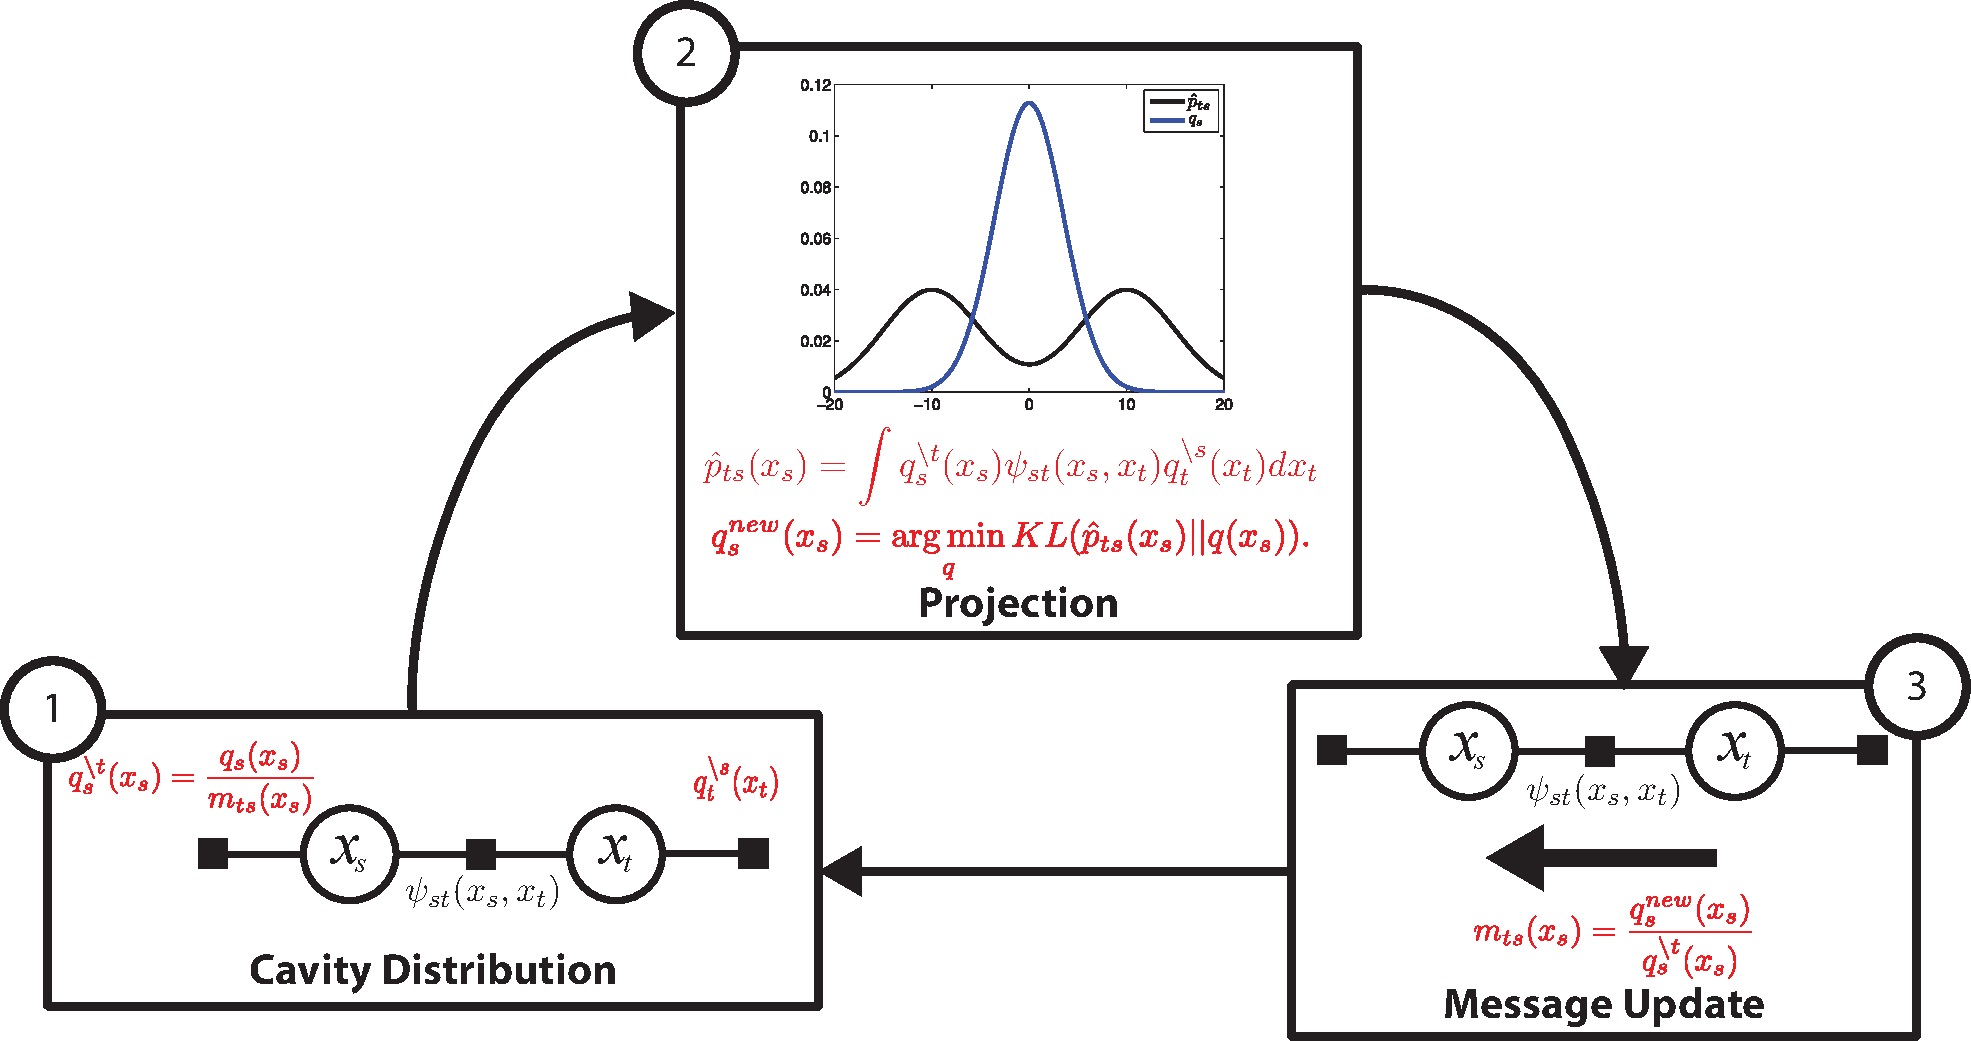
\includegraphics[width=0.9\textwidth]{ep.pdf}
%   \vspace{-3mm}
%   \caption{\small Expectation propagation updates for pairwise
%     MRFs.}
%   \label{fig:ep}
% \end{figure*}

% The message update integral~\eqref{eq:bp_message} constrains BP to
% discrete and Gaussian MRFs.  Expectation Propagation (EP) applies to a
% much broader class of
% models~\cite{minka01uai,heskes_zoeter,wainwright_jordan}, and is made
% possible by exploiting closure properties of the exponential family
% (see Sec.~\ref{sec:expfam}).  For a cleaner presentation we assume a
% pairwise MRF consisting of only pairwise potentials,
% \begin{equation}\label{eq:epmrf}
%   p(x) = \frac{1}{Z} \prod_{(s,t) \in \mathcal{E}} \pot_{st}(x_s,x_t).
% \end{equation}
% This factorization is w.l.o.g.~since node factors $\pot_s$ can always
% be absorbed arbitrarily into a neighboring edge potential.
% Expectation propagation approximates the marginal $p_s(x_s)$ with a
% density in the exponential family defined to be a product of messages,
% \begin{equation}\label{eq:epmarg}
%   \epmarg_s(x_s) = \exp( \langle \theta_s, \phi(x_s) \rangle - \logpart(\theta_s))
%   \propto \prod_{t \in \Gamma(s)} m_{ts}(x_s)
% \end{equation}
% with canonical parameters $\theta_s$, sufficient statistics
% $\phi(x_s)$ and mean parameters $\mu_s = \E[\phi(x_s)]$.  The
% messages $m_{ts}(\cdot)$ belong to the \emph{unnormalized} exponential
% family with parameters $\theta_{ts}$ and a scale factor $\gamma_{ts}$,
% \begin{equation}\label{eq:epmsg}
%   m_{ts}(x_s) = \gamma_{ts} \exp( \langle \theta_{ts}, \phi(x_s)
%   \rangle ).
% \end{equation}

% To update the marginal approximation $\epmarg_s(x_s)$ we first choose
% a factor $\pot_{st}$ and remove the corresponding messages from
% marginals over nodes incident to this factor.  The so-called
% \emph{cavity} is an unnormalized exponential family:
% \begin{equation}\label{eq:ep_cavity}
%   \epmarg_s^{\setminus t}(x_s) = \frac{\epmarg_s(x_s)}{m_{ts}(x_s)} =
%   \gamma_s^{\setminus t} \exp( \langle \theta_s^{\setminus t},
%   \phi(x_s) \rangle).
% \end{equation}
% We form the \emph{augmented distribution} by multiplying the true
% factor $\pot_{st}$ with the corresponding cavity distributions and
% integrating over $x_t$,
% \begin{equation}\label{eq:aug_dist}
%   \hat{p}_{ts}(x_s) = \int \epmarg_s^{\setminus t}(x_s)
%   \pot_{st}(x_s,x_t) \epmarg_t^{\setminus s}(x_t) dx_t.
% \end{equation}
% The augmented distribution~\eqref{eq:aug_dist} is a local
% approximation to the marginal, but is not necessarily in the
% exponential family.  The variational approximation is updated by
% projecting into the exponential family,
% \begin{equation}\label{eq:klproj}
%   \epmarg_s^{new}(x_s) = \argmin_q\; \KL{\hat{p}_{ts}(x_s)}{q(x_s)}.
% \end{equation}
% Using the moment matching property of the exponential family (see
% Sec.~\ref{eq:moment_match}) we update the parameters as,
% \begin{equation}\label{eq:ep_proj}
%   \mu_s^{new} = \mathbb{E}_{\epmarg_s^{new}}[ \phi(x_s) ] =
%   \mathbb{E}_{\hat{p}_{ts}}[ \phi(x_s) ].
% \end{equation}
% One restriction EP imposes is that moments of the augmented
% distribution~\eqref{eq:ep_proj} are computable.  If these integrals
% are not analytic they can be numerically approximated, for example by
% quadrature methods~\cite{zoeter2005gaussian}.  The associated
% canonical parameters $\theta_s^{new}$ can be computed
% from~\eqref{eq:ep_proj} to yield the log-partition
% $\logpart(\theta_s^{new})$, which fully specifies the exponential
% family density.  Finally, we update the message from $t$ to $s$ as,
% \begin{equation}\label{eq:epmsg_update}
%   m_{ts}(x_s) = \frac{ \epmarg_s^{new}(x_s) }{ \epmarg_s^{\setminus t}(x_s) }.
% \end{equation}
% This message update is easily calculated by subtracting canonical
% parameters, $\theta_{ts} = \theta_s^{new} - \theta_s^{\setminus t}$.
% The algorithm proceeds iteratively by updating each factor $\pot_{st}$
% for all $(s,t) \in \mathcal{E}$ in any order.  Convergence is
% determined when the change in message parameters $\theta_{ts}$ falls
% below some specified threshold.


% \section{Example: Labeled LDA}


\bibliography{refs}
\bibliographystyle{abbrvnat}

\end{document}
